
\section{Background}

Tetris (\ref{ref:tetrisGame}) is a puzzle game that involves randomly generated pieces of various shapes that descend onto the board. The player has to complete horizontal lines with the pieces so that the lines would disappear. If the stacked pieces reach the top of the board, the player loses. There are many search algorithms such as the depth-first search, breadth-first search, minimax algorithm \ref{ref:Minimax}, and genetic algorithms \ref{ref:Genetic} that can be applied to solve this game. These search algorithms would benefit from parallel processing and speedup the search for the optimal solution of a single step.

The workload of Tetris is mostly computation-intensive since we would need to search through a huge search space to find the optimal solution under a time constraint. Specifically, we chose a game setting with 7 different shapes of tetrominoes, 4 different orientations, and a game board of 22 rows x 10 columns. Therefore, there are 7 x 4 x 10 = 280 possibilities for a single step in the game. Our search algorithm takes the next two to four blocks into account and calculates the best optimal step.  Thus, for a single step (or a level) of the search space, there are actually 1 x 4 x 10 = 40 possibilities since the next tetromino block is known. For four levels, there would be 40 x 40 x 40 x 40 possible states. Since searching through the 40 possible states on the same level are not data-dependent on each other, it would benefit greatly from parallelization. However, searching and computing the scores of block placement on subsequent levels would depend on the game state of previous levels. Therefore, we can only perform parallelization across states on the same level. That still amounts to 40 states for the first level, 40 x 40 on the second level, and so on. Moreover, we found that there are some duplicate states when simply conducting naive parallelization across states on the same level. One such example is that the four orientations of a square tetromino is calculated as four different states when they are essentially the same. Pruning these states would cause workload imbalance, so we came up with various optimizations to alleviate the problem which we would introduce in the following sections.

\begin{figure}[h]
	\centering
	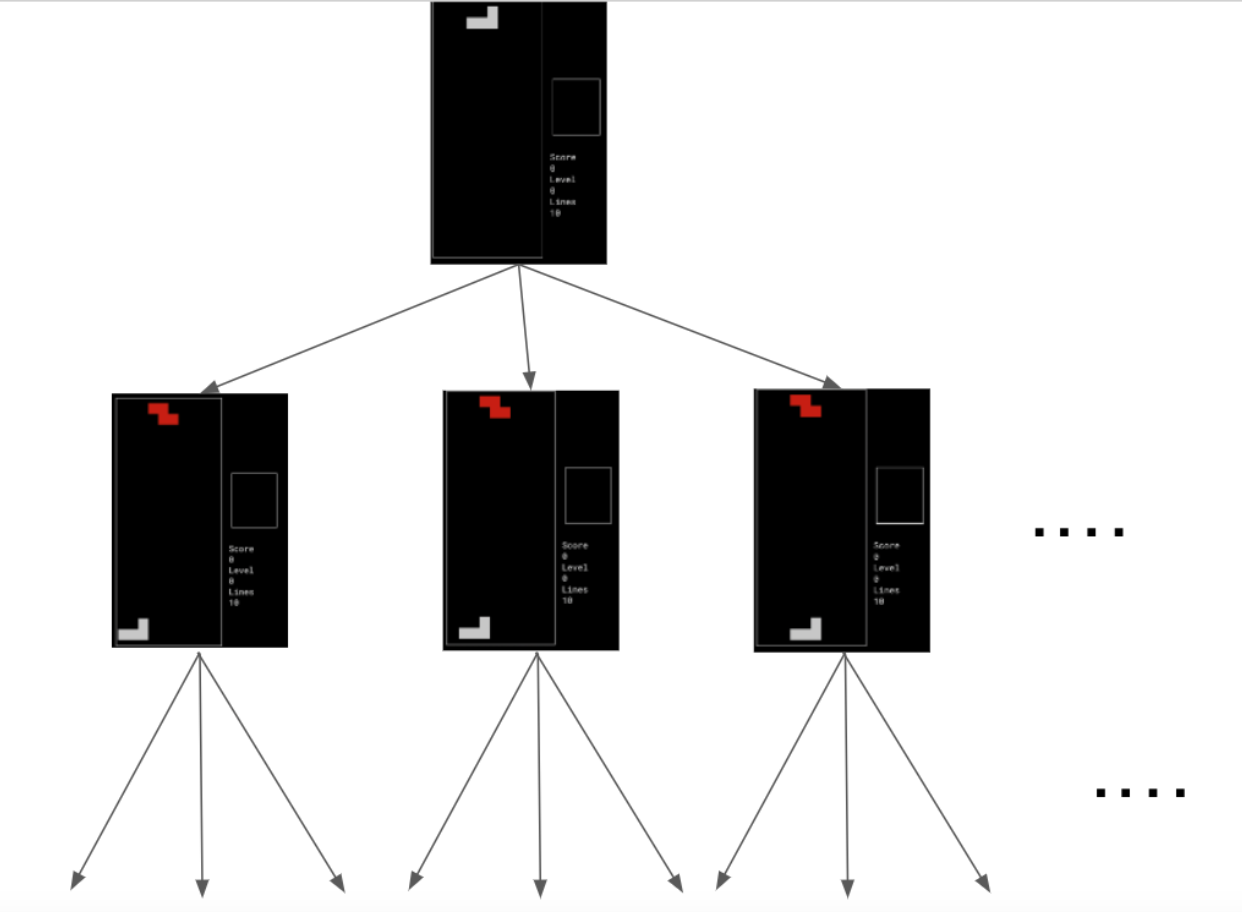
\includegraphics[width=0.3\textwidth]{search_space.png}
	\vspace{-1em}
	\caption{Tetris game search tree.}
	\label{fig:search_space}
\end{figure}

To evaluate a state for the search algorithm, we defined some evaluation metrics related to the tetris game such as the maximum height of the stacked blocks, holes in the game board not filled by blocks and lines cleared. The evaluation score is a weighted sum of these metrics, and is used to help the algorithm select the optimal position and orientation of the next move. We conducted experiments to obtain a set of weights that performed the best on achieving the highest score, which is used in guiding our search algorithms. Since this is not related to the parallelization of the search algorithms, we omit the details in our report.

\begin{figure}[h]
	\centering
	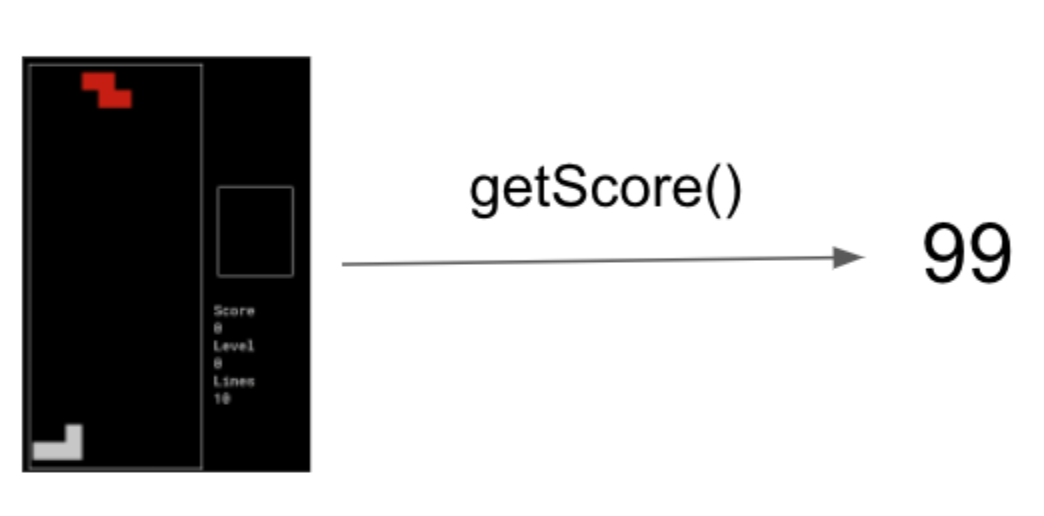
\includegraphics[width=0.2\textwidth]{score.png}
	\vspace{-1em}
	\caption{Score of tetris game state.}
	\label{fig:score}
\end{figure}

Our implementation is based on a tetris game repository (\ref{ref:tetrisRepo}) implemented in C on Github. We adopted its code for the game-play and game settings. Given the next four blocks to be dropped, we implemented solvers that calculate the next best orientation and position to place a tetris block, and supply it to the game. 

\begin{comment}

\subsection{Selecting a Template (Heading 2)}

First, confirm that you have the correct template for your paper size. This template has been tailored for output on the US-letter paper size. Please do not use it for A4 paper since the margin requirements for A4 papers may be different from Letter paper size.

\subsection{Maintaining the Integrity of the Specifications}

The template is used to format your paper and style the text. All margins, column widths, line spaces, and text fonts are prescribed; please do not alter them. You may note peculiarities. For example, the head margin in this template measures proportionately more than is customary. This measurement and others are deliberate, using specifications that anticipate your paper as one part of the entire proceedings, and not as an independent document. Please do not revise any of the current designations.

\end{comment}